\documentclass[sigconf,anonymous,review]{acmart}
\usepackage{popets}

% Copyright
\setcopyright{popets}
\copyrightyear{YYYY}

% Issue info
\acmYear{YYYY}
\acmVolume{YYYY}
\acmNumber{X}
\acmDOI{XXXXXXX.XXXXXXX}
\acmISBN{}
\acmConference{Proceedings on Privacy Enhancing Technologies}
\settopmatter{printacmref=false,printccs=false,printfolios=true}

\begin{document}

% The "title" command has an optional parameter, allowing the author to define a
% "short title" to be used in page headers.
\title[The Name of the Title Is Hope]{The Name of the Title Is Hope: This is the Longer Version of the Given Title}

% The "author" command and its associated commands are used to define the
% authors and their affiliations.
\author{Ben Trovato}
\orcid{1234-5678-9012}
\affiliation{%
  \institution{Institute for Clarity in Documentation}
  \city{Dublin}
  \state{Ohio}
  \country{USA}}
\email{trovato@corporation.com}

\author{Lars Th{\o}rv{\"a}ld}
\affiliation{%
  \institution{The Th{\o}rv{\"a}ld Group}
  \city{Hekla}
  \country{Iceland}}
\email{larst@affiliation.org}

\author{Valerie B\'eranger}
\affiliation{%
  \institution{Inria Paris-Rocquencourt}
  \city{Rocquencourt}
  \country{France}
}
\email{valerie@affiliation.org}

\author{Aparna Patel}
\affiliation{%
 \institution{Rajiv Gandhi University}
 \city{Doimukh}
 \state{Arunachal Pradesh}
 \country{India}}
\email{aparnap@rgu.ac.in}

% By default, the full list of authors will be used in the page headers. Often,
% this list is too long, and will overlap other information printed in the page
% headers. This command allows the author to define a more concise list of
% authors' names for this purpose.
\renewcommand{\shortauthors}{Trovato et al.}

\begin{abstract}
  Abstract goes here in the dedicated environment.
\end{abstract}

% Keywords. The author(s) should pick words that accurately describe the work
% being presented. Separate the keywords with commas.
\keywords{datasets, neural networks, gaze detection, text tagging}

\maketitle

\section{Introduction -- Scope of PoPETs}

Papers must present novel research into privacy-enhancing technologies (PETs)
and the social, cultural, legal, or situational contexts in which they are used.
Interdisciplinary work is welcome as long as it clearly shows how the
contributions impact PETs.

Please follow the guidelines given below to ensure that your submission passes
desk review and receives a full review by the program committee. You may ask the
chairs for clarification of scope \emph{before} the submission deadline.

\begin{itemize}
  \item Papers must have strong ties to privacy in digital systems.
  \item The core contribution must be relevant to real-world privacy applications.
  \begin{itemize}
    \item The \textbf{first page must clearly state how the work is relevant to
    real-world privacy applications}.
    \item Relevance to real-world privacy applications must also be present throughout the entire paper by dedicating a substantial portion of the submission to work that is traditionally considered practical or applied.
  \end{itemize}
  \item For contributions of theoretical nature (e.g., improvements on
  cryptographic primitives or improvements on differential privacy), the paper
  should provide details about how the proposed advances would be integrated
  into a real-world application.
  \item Improvements motivated by real applications, but presented in isolation
    without connection to those applications, do not demonstrate relevance in
    practice and are therefore out of scope.
    \item Papers with empirical evaluations must show a clear connection to
    privacy and to real-world applications.
  \item Evaluations that are based on purely synthetic datasets, or on
    non-privacy-relevant datasets (e.g., MNIST, CIFAR, or SVHN) must contain a
    well-marked paragraph explaining why the results of the evaluation can be
    extrapolated to real-world use cases where privacy is of relevance.
    \item Papers that treat privacy as a superficial application domain (e.g.,
    if the only relationship to privacy is a privacy-related dataset) do not
    demonstrate relevance to real-world privacy problems and are therefore out
    of scope.
\end{itemize}

\section{Anonymization of Submission}

All submitted papers will be judged based on their quality and relevance through
double-blind reviewing, where the identities of the authors are withheld from
the reviewers. As an author, you are required to make a good-faith effort to
preserve the anonymity of your submission, while at the same time allowing the
reader to fully grasp the context of related past work, including your own. It
is recognized that, at times, information regarding the identities of authors
may become public outside the submission process (e.g., if a pre-print is
published as a technical report or on a pre-print server). The PC will ignore
this external information.

Minimally, please take the following steps when preparing your submission:

\begin{itemize}
  \item Remove the names and affiliations of authors from the title page.
  Handled by using \verb|[anonymous,review]| in the \verb|documentclass| at the
  top of this template.
  \item Remove acknowledgment of identifying names and funding sources. The
  acknowledgement section is also hidden by \verb|[anonymous,review]|.
  \item Remove references to your institution, for example in survey materials
  or in git repositories.
  \item Remove references to other external content that obviously deanonymizes
  the authors, e.g., an author's webpage or a git repo with author attribution.
  If it is important to reference such material, consider setting up a cloned
  version with identifying information removed, perhaps using anonymization
  tools such as \url{https://anonymous.4open.science}.
  \item Use care in referring to related work, particularly your own. Do not
  omit references to provide anonymity, as this leaves the reviewer unable to
  grasp the context. Instead, reference your past work in the third person, just
  as you would any other piece of related work by another author.
\end{itemize}

\section{No Format Modifications}

Authors should use the provided template without modifying the overall format or
``look and feel'' produced by the template. Papers that, in the chair's
assessment, exploit underspecified formatting criteria (e.g., columns),
manipulate other document properties (e.g., page layout, spacing, use the
\verb|\vspace| command, fonts, figures and tables, headings), remove the
copyright block (CC-BY-4.0 text, including image) on the first page, etc., in an
attempt to gain an unfair advantage \textbf{will be desk-rejected}.

\section{Sectioning Commands}

Your work should use standard \LaTeX\ sectioning commands: \verb|section|,
\verb|subsection|, \verb|subsubsection|, and \verb|paragraph|. They should be
numbered; do not remove the numbering from the commands.

\section{Tables}

The ``\verb|acmart|'' document class includes the ``\verb|booktabs|'' package
--- \url{https://ctan.org/pkg/booktabs} --- for preparing high-quality tables.

Table captions are placed {\itshape above} the table.

Immediately following this sentence is the point at which Table~\ref{tab:freq}
is included in the input file; compare the placement of the table here with the
table in the printed output of this document.

\begin{table}
  \caption{Frequency of Special Characters}
  \label{tab:freq}
  \begin{tabular}{ccl}
    \toprule
    Non-English or Math&Frequency&Comments\\
    \midrule
    \O & 1 in 1,000& For Swedish names\\
    $\pi$ & 1 in 5& Common in math\\
    \$ & 4 in 5 & Used in business\\
    $\Psi^2_1$ & 1 in 40,000& Unexplained usage\\
  \bottomrule
\end{tabular}
\end{table}

To set a wider table, which takes up the whole width of the page's live area,
use the environment \textbf{table*} to enclose the table's contents and the
table caption.

\begin{table*}
  \caption{Some Typical Commands}
  \label{tab:commands}
  \begin{tabular}{ccl}
    \toprule
    Command &A Number & Comments\\
    \midrule
    \texttt{{\char'134}author} & 100& Author \\
    \texttt{{\char'134}table}& 300 & For tables\\
    \texttt{{\char'134}table*}& 400& For wider tables\\
    \bottomrule
  \end{tabular}
\end{table*}

Always use midrule to separate table header rows from data rows, and use it only
for this purpose. This enables assistive technologies to recognise table headers
and support their users in navigating tables more easily.

\section{Math Equations}
You may want to display math equations in three distinct styles: inline,
numbered or non-numbered display.  Each of the three are discussed in the next
sections.

\subsection{Inline (In-text) Equations}
A formula that appears in the running text is called an inline or in-text
formula.  It is produced by the \textbf{math} environment, which can be invoked
with the usual \texttt{{\char'134}begin\,\ldots{\char'134}end} construction or
with the short form \texttt{\$\,\ldots\$}. You can use any of the symbols and
structures, from $\alpha$ to $\omega$, available in \LaTeX~\cite{Lamport:LaTeX};
this section will simply show a few examples of in-text equations in context.
Notice how this equation:
\begin{math}
  \lim_{n\rightarrow \infty}x=0
\end{math},
set here in in-line math style, looks slightly different when set in display
style.  (See next section).

\subsection{Display Equations}
A numbered display equation---one set off by vertical space from the text and
centered horizontally---is produced by the \textbf{equation} environment. An
unnumbered display equation is produced by the \textbf{displaymath} environment.

Again, in either environment, you can use any of the symbols and structures
available in \LaTeX\@; this section will just give a couple of examples of
display equations in context.  First, consider the equation, shown as an inline
equation above:
\begin{equation}
  \lim_{n\rightarrow \infty}x=0
\end{equation}
Notice how it is formatted somewhat differently in the \textbf{displaymath}
environment.  Now, we'll enter an unnumbered equation:
\begin{displaymath}
  \sum_{i=0}^{\infty} x + 1
\end{displaymath}
and follow it with another numbered equation:
\begin{equation}
  \sum_{i=0}^{\infty}x_i=\int_{0}^{\pi+2} f
\end{equation}
just to demonstrate \LaTeX's able handling of numbering.

\section{Figures}

The ``\verb|figure|'' environment should be used for figures. One or more images
can be placed within a figure. If your figure contains third-party material, you
must clearly identify it as such, as shown in the example below.
\begin{figure}[ht]
  \centering
  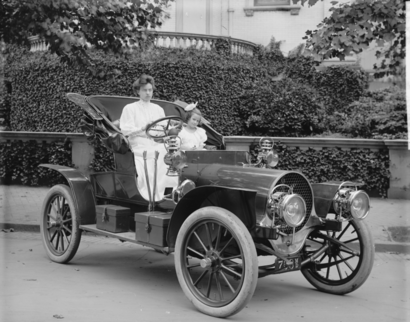
\includegraphics[width=\linewidth]{sample-franklin}
  \caption{1907 Franklin Model D roadster. Photograph by Harris \& Ewing, Inc.
    [Public domain], via Wikimedia Commons. (\url{https://goo.gl/VLCRBB}).}
    \Description{A woman and a girl in white dresses sit in an open car.}
\end{figure}

Your figures should contain a caption which describes the figure to the reader.
Figure captions are placed {\itshape below} the figure.

Every figure should also have a figure description unless it is purely
decorative. These descriptions convey what's in the image to someone who cannot
see it. They are also used by search engine crawlers for indexing images, and
when images cannot be loaded.

A figure description must be unformatted plain text less than 2000 characters
long (including spaces).  {\bfseries Figure descriptions should not repeat the
figure caption – their purpose is to capture important information that is not
already provided in the caption or the main text of the paper.} For figures that
convey important and complex new information, a short text description may not
be adequate. More complex alternative descriptions can be placed in an appendix
and referenced in a short figure description. For example, provide a data table
capturing the information in a bar chart, or a structured list representing a
graph.  For additional information regarding how best to write figure
descriptions and why doing this is so important, please see
\url{https://www.acm.org/publications/taps/describing-figures/}.

\section{Citations and Bibliographies}

The use of BibTeX for the preparation and formatting of one's references is
strongly recommended. Authors' names should be complete --- use full first names
(``Donald E. Knuth'') not initials (``D. E. Knuth'') --- and the salient
identifying features of a reference should be included: title, year, volume,
number, pages, article DOI, etc.

Some examples.  A paginated journal article \cite{Abril07}, an enumerated
journal article \cite{Cohen07}, a reference to an entire issue \cite{JCohen96},
a monograph (whole book) \cite{Kosiur01}, a monograph/whole book in a series
(see 2a in spec. document) \cite{Harel79}, a divisible-book such as an anthology
or compilation \cite{Editor00} followed by the same example, however we only
output the series if the volume number is given \cite{Editor00a} (so Editor00a's
series should NOT be present since it has no vol. no.), a chapter in a divisible
book \cite{Spector90}, a chapter in a divisible book in a series
\cite{Douglass98}, a multi-volume work as book \cite{Knuth97}, a couple of
articles in a proceedings (of a conference, symposium, workshop for example)
(paginated proceedings article) \cite{Andler79, Hagerup1993}, a proceedings
article with all possible elements \cite{Smith10}, an example of an enumerated
proceedings article \cite{VanGundy07}, an informally published work
\cite{Harel78}, a couple of preprints \cite{Bornmann2019, AnzarootPBM14}, a
doctoral dissertation \cite{Clarkson85}, a master's thesis: \cite{anisi03}, an
online document / world wide web resource \cite{Thornburg01, Ablamowicz07,
Poker06}, a video game (Case 1) \cite{Obama08} and (Case 2) \cite{Novak03} and
\cite{Lee05} and (Case 3) a patent \cite{JoeScientist001}, work accepted for
publication \cite{rous08}, 'YYYYb'-test for prolific author \cite{SaeediMEJ10}
and \cite{SaeediJETC10}. Other cites might contain 'duplicate' DOI and URLs
(some SIAM articles) \cite{Kirschmer:2010:AEI:1958016.1958018}. Boris / Barbara
Beeton: multi-volume works as books \cite{MR781536} and \cite{MR781537}. A
couple of citations with DOIs:
\cite{2004:ITE:1009386.1010128,Kirschmer:2010:AEI:1958016.1958018}. Online
citations: \cite{TUGInstmem, Thornburg01, CTANacmart}. Artifacts: \cite{R} and
\cite{UMassCitations}.

% This is the end of the main body of the paper. Note the page limit of 12
% typeset pages for a normal submission, 13 pages for a revision.
% Acknowledgements, Ethical Considerations, Open Science, AI Use, References,
% and the Appendix are all outside of the main body.

\appendix

\begin{acks}
The acknowledgments section is defined using the "acks" environment (and NOT an
unnumbered section). This ensures the proper identification of the section in
the article metadata, and the consistent spelling of the heading. Does NOT count
towards page limit. NOT shown (as intended) for anonymous submission. Only edit
for the camera-ready.

Identification of funding sources and other support, and thanks to individuals
and groups that assisted in the research and the preparation of the work should
be included.
\end{acks}

\begin{ethics}
Mandatory section for PoPETs 2027. Does NOT count towards page limit. MUST have
exactly this title and placement (between acknowledgements and references) or
risk desk rejection.

This section should include a justification of the ethics of the work and
information about whether the work was submitted to an external ethics panel
such as an IRB or the Tor Research Safety Board. Research that is deemed to not
have met adequate ethical standards may be rejected on those grounds. Authors
are encouraged to contact PC chairs before submitting to clarify any doubts.
\end{ethics}

\begin{openscience}
Mandatory section for PoPETs 2027. Does NOT count towards page limit. MUST have
exactly this title and placement (between acknowledgements and references) or
risk desk rejection.

To encourage reproducibility, PETS champions open science:
\begin{itemize}
  \item If you provide any research artifacts for the submission, please link
  them here. Make sure that identifying information is removed, perhaps using
  anonymization tools such as \url{https://anonymous.4open.science}.
  \item If you plan to share research artifacts upon acceptance, please briefly
  describe the artifacts here.
  \item If you do not plan to release any research artifacts, please briefly
  justify the decision here.
\end{itemize}

Note that this part is distinct from the artifact review that takes place after
a paper is accepted.
\end{openscience}

\begin{ai}
Mandatory section for PoPETs 2027. Does NOT count towards page limit. MUST have
exactly this title and placement (between acknowledgements and references) or
risk desk rejection.

The goal of this section is to disclose the use of any AI-based tools (e.g.,
ChatGPT, Cursor, Claude Code, FigureLabs) used in the process of producing the
paper. If you have not used any AI-based tools, do not remove this section.
Instead, add a single sentence, ``AI-based tools were not used in this work,''
or similar. 

If you have used AI-based tools to improve writing, please acknowledge it here.
For example, ``The authors used generative AI-based tools to revise the text,
improve flow, and correct any typos, grammatical errors, and awkward phrasing.''
If figures have been significantly or completely generated with AI-based tools,
list the figures here and attribute the AI use in the caption of each figure.

If you used AI-based tools as part of your research methodology, describe it
thoroughly in the text of the paper, and simply acknowledge it here. For
example, "As described in Section 4, AI-based tools were used to assist with
data labeling by generating initial annotations.''

Describe any other AI use here. For example, ``AI-based tools were used to
search for additional related work'', ``AI-based tools were used for
pre-submission review'', or ``AI-based tools were used in the artifact
development and to verify that the methods section of the paper correctly
describes the codebase''. We encourage transparency to help reviewers assess
your work and for fellow scientists to learn about the ethical and constructive
use of AI in the scientific process.

Finally, if you answered yes to any of the cases above or have used AI in any
other way, you are responsible for the accuracy, originality, and integrity of
the output of all AI-based tools. As such, indicate this in this section. For
example, ``We have manually verified and are responsible for the accuracy,
originality, and integrity of the output of all AI-based tools.''
\end{ai}

% The next two lines define the bibliography style to be used (do not change),
% and the bibliography file (use as many or few as you wish).
\bibliographystyle{ACM-Reference-Format}
\bibliography{sample-base}

\section{An Appendix Section}
\label{appendix:first}
If your work has an appendix, this is the place to put it. Note that in the
appendix, sections are lettered, not numbered. This document has two appendices,
Appendix~\ref{appendix:first} and Appendix~\ref{appendix:second}, demonstrating
the section and subsection identification method.

\subsection{Part One}

Lorem ipsum dolor sit amet, consectetur adipiscing elit.

\subsection{Part Two}

Etiam commodo feugiat nisl pulvinar pellentesque. Etiam auctor sodales ligula,
non varius nibh pulvinar semper. Suspendisse nec lectus non ipsum convallis
congue hendrerit vitae sapien. Donec at laoreet eros.

\section{Online Resources}
\label{appendix:second}
Nam id fermentum dui. Suspendisse sagittis tortor a nulla mollis, in pulvinar ex
pretium. Sed interdum orci quis metus euismod, et sagittis enim maximus.
Vestibulum gravida massa ut felis suscipit congue. Nam interdum magna at lectus
dignissim, ac dignissim lorem rhoncus. Maecenas eu arcu ac neque placerat
aliquam. Nunc pulvinar massa et mattis lacinia.

\end{document}
\endinput
